\section{\textit{Indexing}}
% Kita dapat mencari halaman yang berisikan suatu topik atau kata kunci pada sebuah buku teks dengan melihat indeks sebuah buku. Indeks disusun secara terurut dan mengurangi usaha untuk mencari suatu hal yang diinginkan oleh penggunanya. Secara umum, indeks pada sebuah file di sebuah basis data berlaku sama pada indeks di buku teks, \parencite{database}.

% Konsep \textit{caching} sendiri adalah menyimpan data yang sering diakses pada level cache atau memori yang lebih dekat dengan CPU agar dapat diakses dengan cepat saat ingin melakukan pencarian, lihat gambar \ref{fig:cache-level}. \textit{Cache} sendiri biasanya memiliki ruang yang terbatas sehingga biasanya membuang data yang sudah tidak diakses sehingga jika dibutuhkan harus dicari ke \textit{storage}. Konsep ini ditiru oleh basis data dan aplikasi \textit{information retrieval} untuk mempercepat proses pencarian dengan memanfaatkan \textit{indexing} untuk mencari (lihat gambar \ref{fig:cache-app}) dan \textit{caching} untuk mengembalikan data yang sering diakses dengan memanfaatkan memori.

% \begin{figure}[h]
%     \centering
%     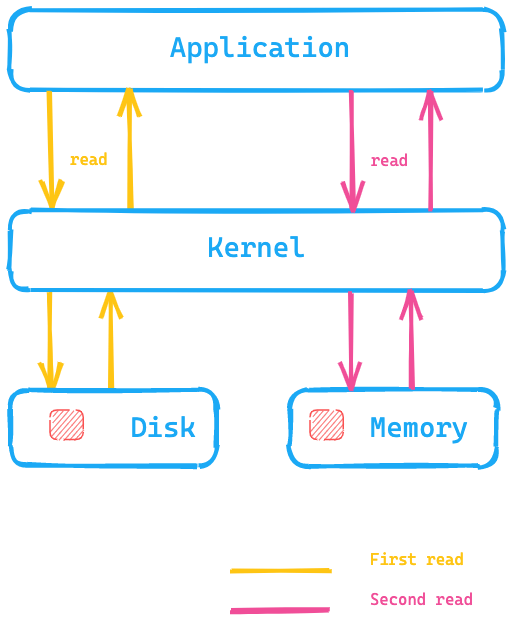
\includegraphics[width=0.5\textwidth]{chapter-2/cache-app.png}
%     \caption{Prinsip Cache pada Aplikasi}
%     \label{fig:cache-app}
% \end{figure}

% \begin{figure}[h]
%     \centering
%     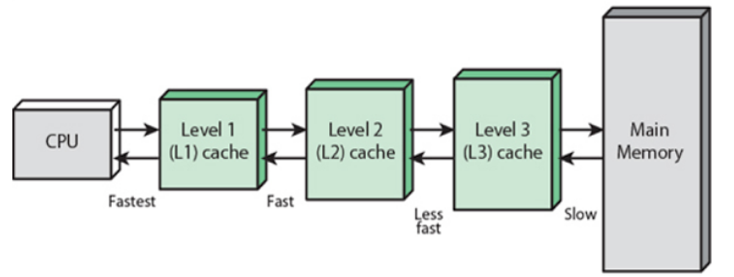
\includegraphics[width=0.5\textwidth]{chapter-2/cache-memory.jpeg}
%     \caption{Level-level pada Cache}
%     \label{fig:cache-level}
% \end{figure}